\section{The \model Architecture}\label{sec:model}


In the section, we present the \model model. 
Figure \ref{fig:model} illustrates the overall architecture. 
Given a pair of video and text input,  we design a \textbf{3D causal VAE} to compress the video into the latent space, and the latents are then patchified and unfolded into a long sequence denoted as $z_{\text{vision}}$. 
Simultaneously, we encode the textual input into text embeddings $z_{\text{text}}$ using T5~\citep{raffel2020exploring}. 
Subsequently, $z_{\text{text}}$ and $z_{\text{vision}}$ are concatenated along the sequence dimension. 
The concatenated embeddings are then fed into a stack of \textbf{expert transformer} blocks.
Finally, the model output are unpatchified to restore the original latent shape, which is then decoded using a 3D causal VAE decoder to reconstruct the video. 
We illustrate the technical design of the 3D causal VAE and expert transfomer in detail.


\begin{figure}[h]
\begin{center}
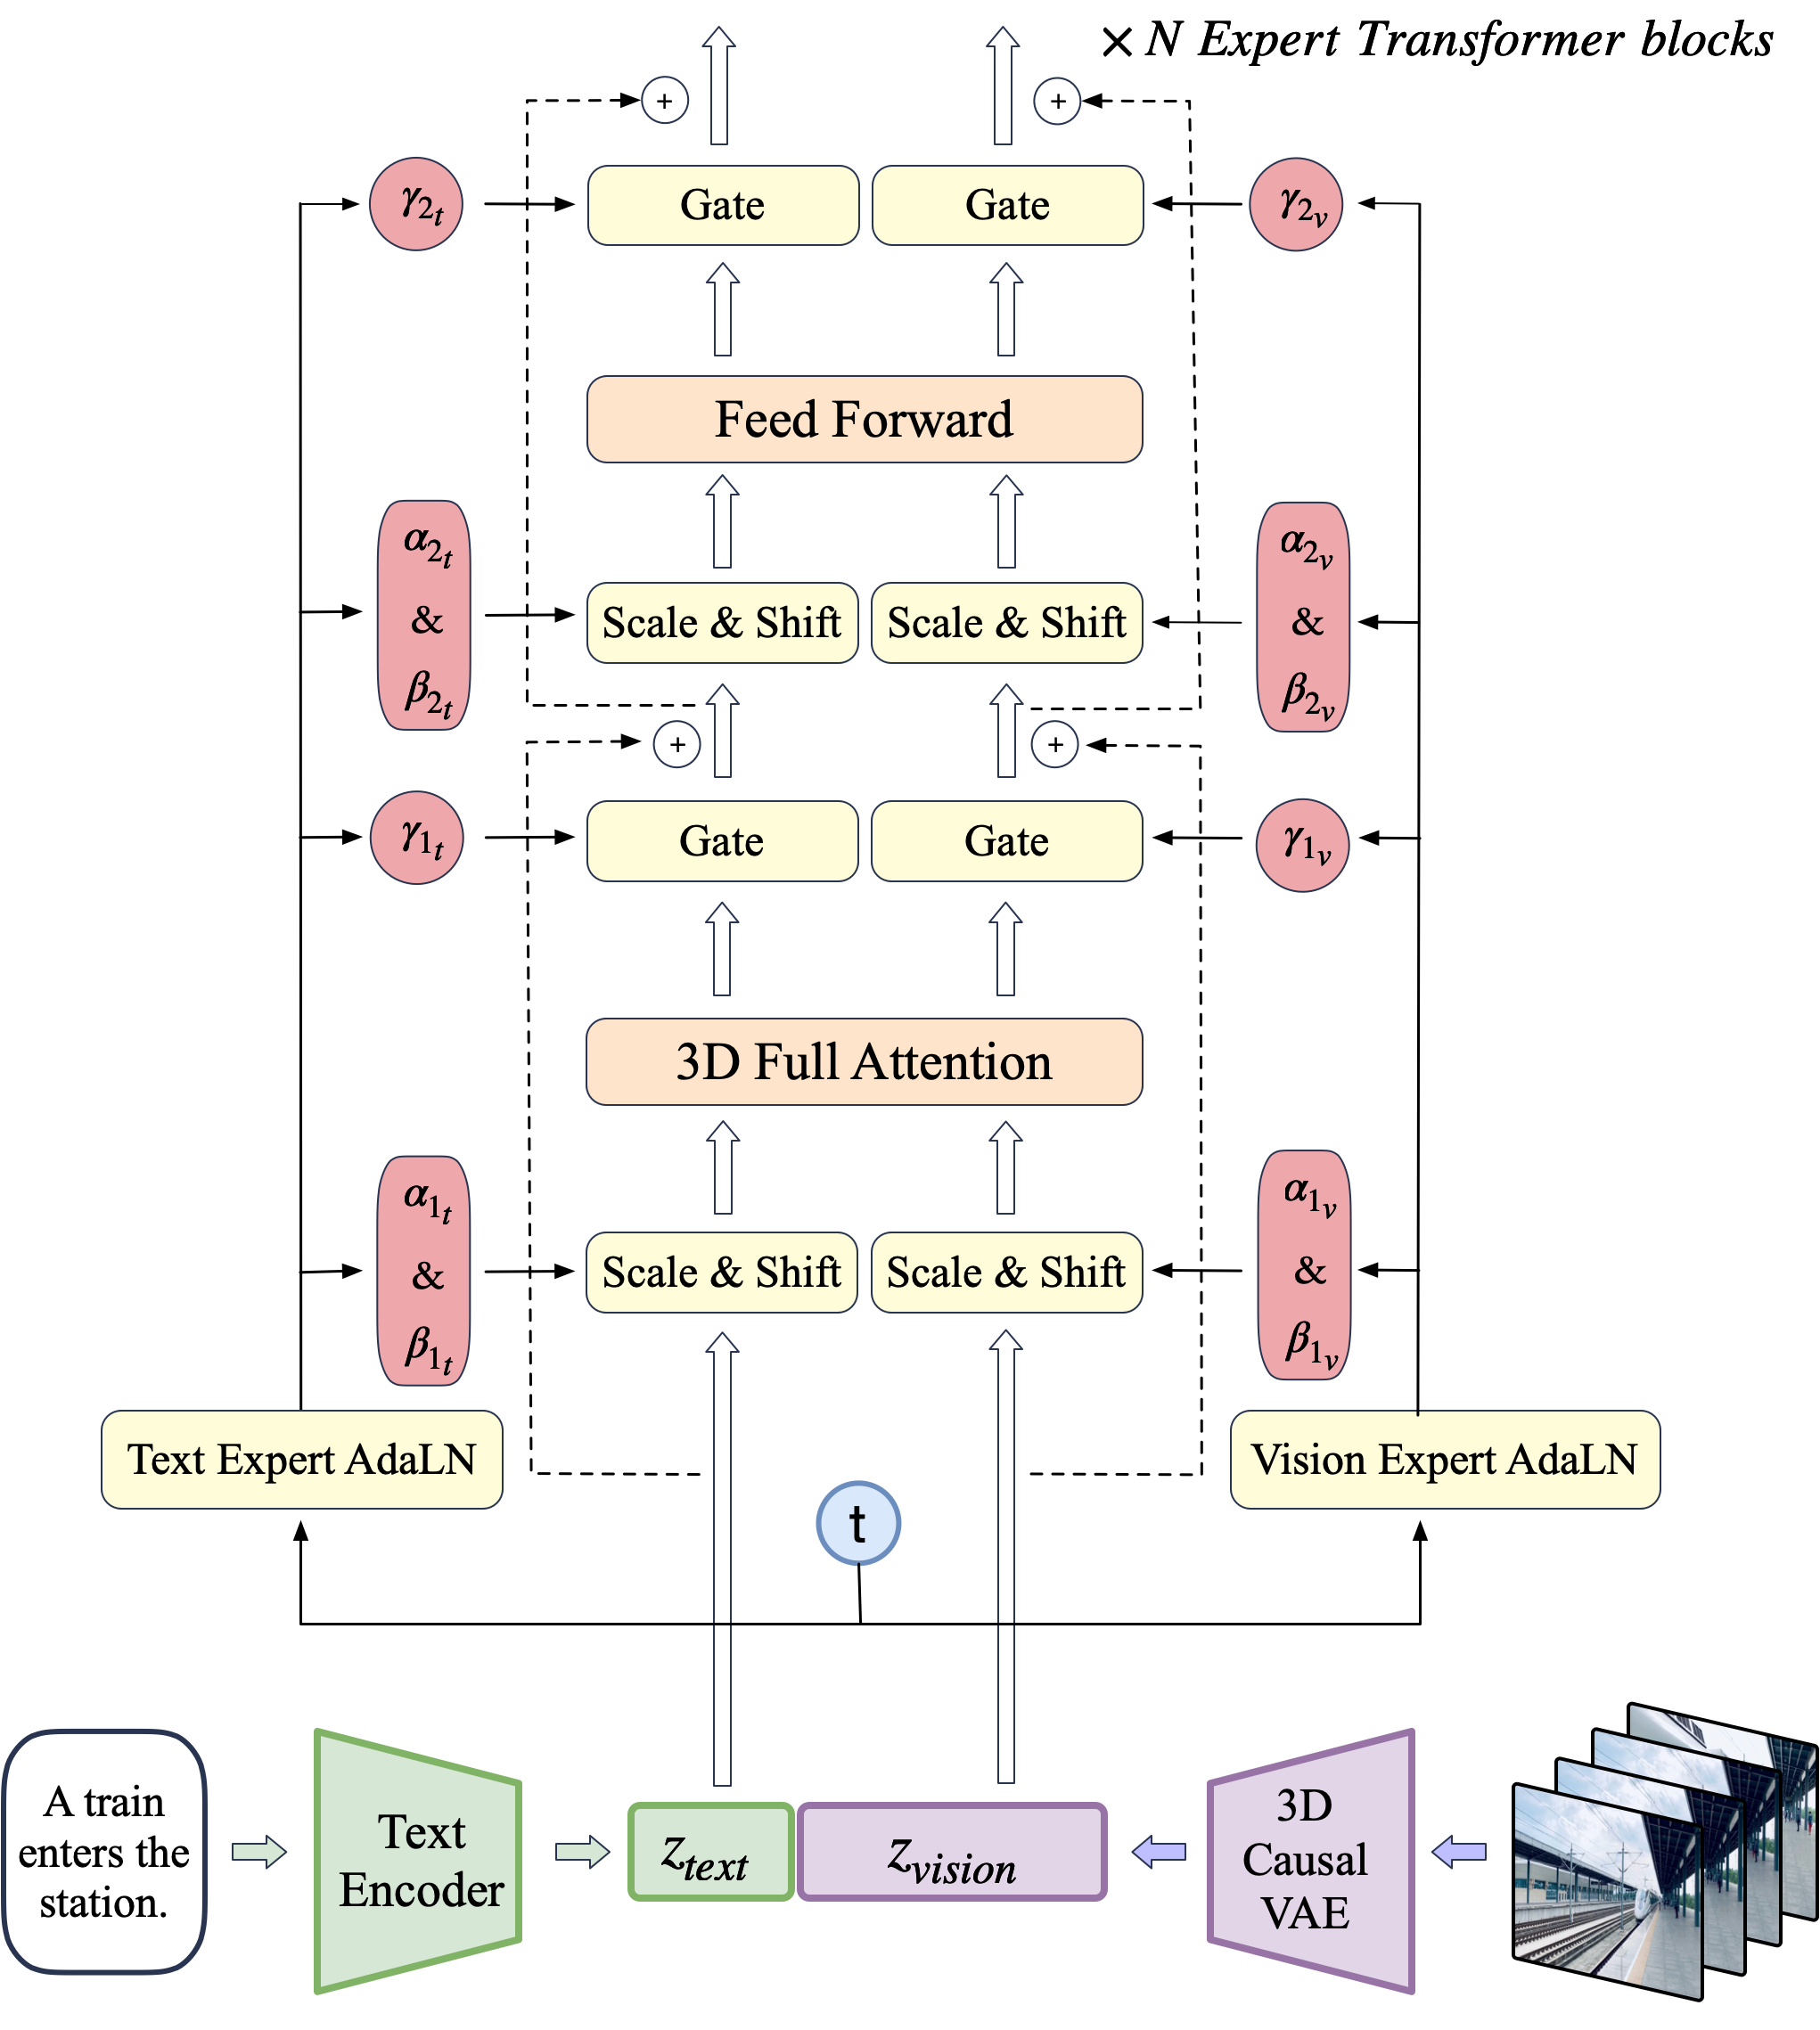
\includegraphics[width=0.7\linewidth]{images/transformer.png}
\end{center}
\caption{\textbf{The overall architecture of \model.} }
\label{fig:model}
\end{figure}



\subsection{3D Causal VAE} 

%Compared to image data, 

Videos encompass not only spatial information but also substantial temporal information, usually resulting in orders of magnitude more data volumes than images.  
To tackle the computational challenge of modeling video data, we propose to implement a video compression module based on 3D Variational Autoencoders (3D VAEs)~\citep{yu2023language}.
%Our 3D VAE
The idea is to incorporate three-dimentional convolutions to compress videos both spatially and temporally. 
This can help achieve a higher compression ratio with largely improved quality and continuity of video reconstruction when compared to previous image VAEs~\citep{rombach2022high, esser2021taming}. 
\begin{figure}[h]
\begin{center}
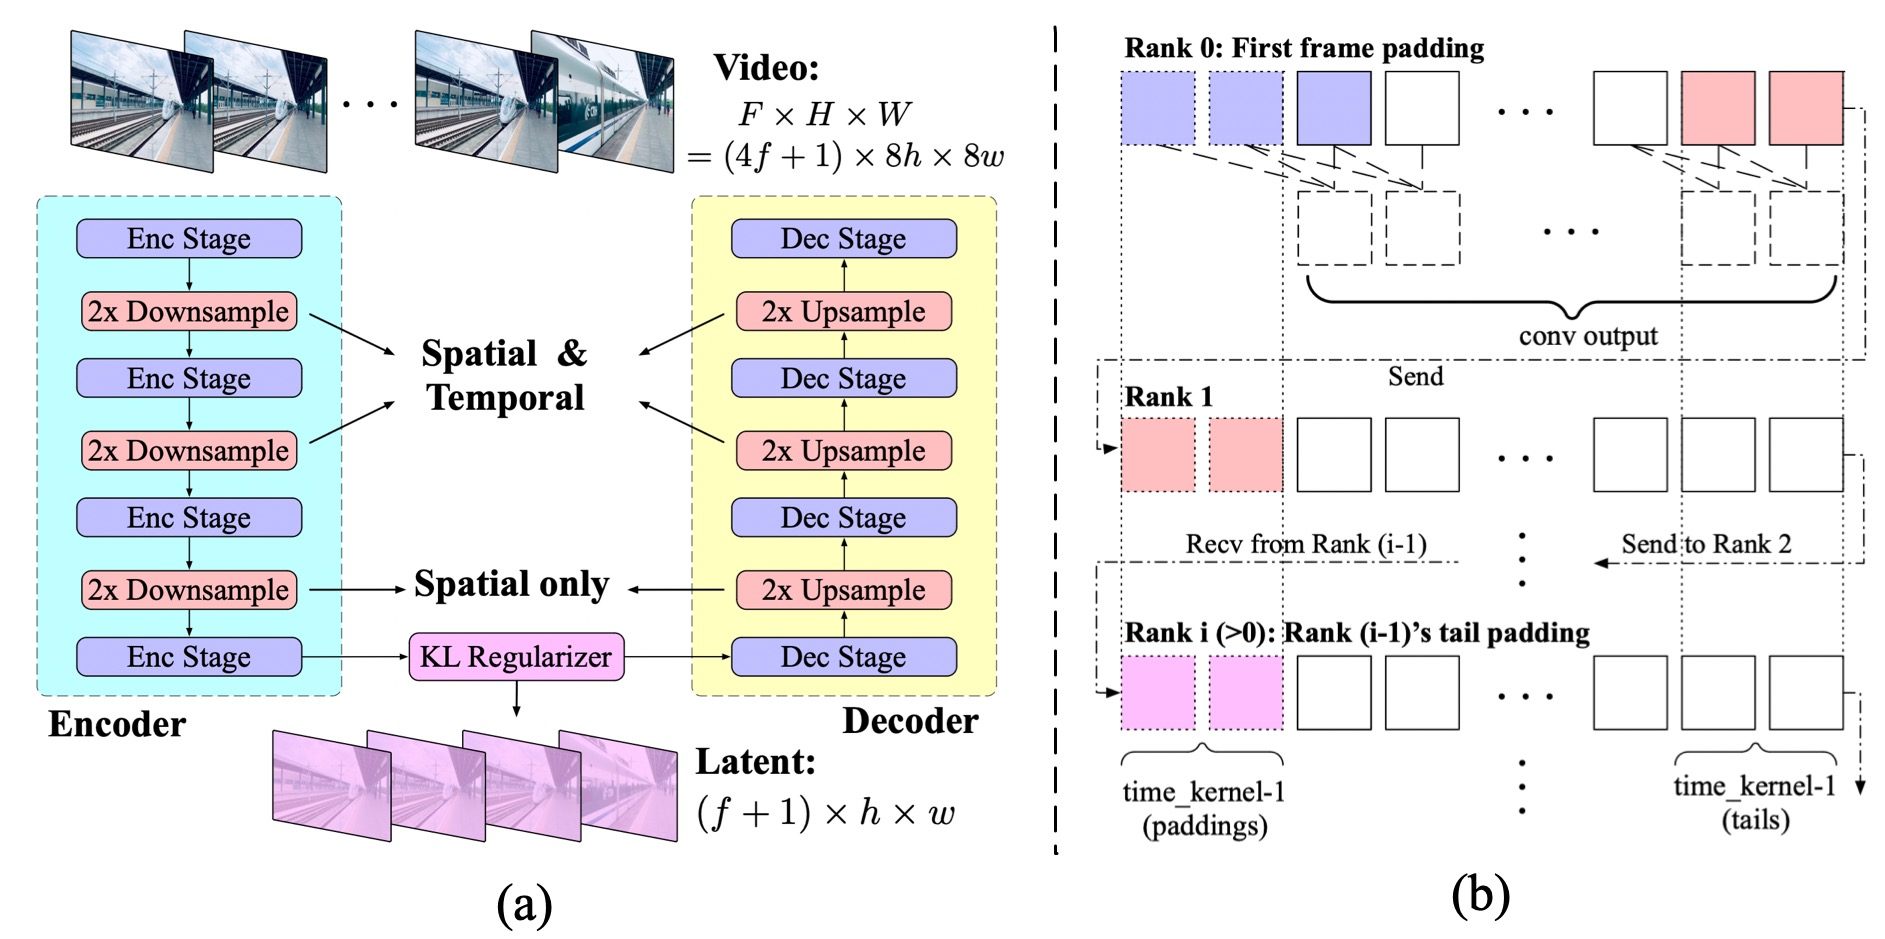
\includegraphics[width=\linewidth]{images/3dvae_combined.jpg}
\end{center}
\caption{(a) The structure of the 3D VAE in \model. It comprises an encoder, a decoder and a latent space regularizer, achieving a 4$\times$8$\times$8 compression from pixels to the latents. (b) The context parallel implementation on the temporally causal convolution.}
\label{fig:3dvae_combined}
\end{figure}

Figure~\ref{fig:3dvae_combined} (a) shows the structure of the proposed 3D VAE. 
It comprises an encoder, a decoder and a latent space regularizer. 
The Gaussian latent space is constrained by a Kullback-Leibler (KL) regularizer.
The encoder and decoder consist of four symmetrically arranged stages, respectively performing 2$\times$ downsampling and upsampling by the interleaving of ResNet block stacked stages. 
The first two rounds of downsampling and the last two upsampling involve both the spatial and temporal dimensions, while the last round only applies spatial sampling. 
This enables the 3D VAE to achieve a 4$\times$ compression in the temporal dimension and an 8$\times$8 compression in the spatial dimension. 
In total, this achieves a 4$\times$8$\times$8 compression from pixels to the latents. 

We adopt the temporally causal convolution~\citep{yu2023language}, which places all the paddings at the beginning of the convolution space, as shown in Figure~\ref{fig:3dvae_combined} (b). 
This ensures the future information not to influence the present or past predictions. 
Given that processing videos with a large number of frames introduces excessive GPU memory usage, we apply context parallel at the temporal dimension for 3D convolution to distribute computation among multiple devices. 
As illustrated by Figure~\ref{fig:3dvae_combined} (b), due to the causal nature of the convolution, each rank simply sends a segment of length $k-1$ to the next rank, where $k$ indicates the temporal kernel size. 
This results in relatively low communication overhead.

During actual implementation, we first train a 3D VAE on lower resolutions and fewer frames to save computation. 
We observe that the encoding of larger resolution generalizes naturally, while extending the number of frames to be encoded does not work as seamlessly. 
Therefore, we conduct a two-stage training process by first training on short videos and finetuning by context parallel on long videos. 
Both stages of training utilize a weighted combination of the L2 loss, LPIPS~\citep{zhang2018unreasonable} perceptual loss, and GAN loss from a 3D discriminator.
